\documentclass[12pt]{article}
\usepackage{fullpage}

\usepackage[T1]{fontenc}
\usepackage[utf8]{inputenc}
\usepackage{lmodern}
\usepackage{microtype}
\usepackage{amsmath,amssymb,amsthm}
\usepackage{mathtools}
\usepackage{graphicx}
\usepackage{booktabs}
\usepackage{hyperref}
\usepackage{url}
\usepackage{xcolor}
\usepackage[shortlabels]{enumitem}
\usepackage{amsfonts}
\usepackage{tikz}
\usetikzlibrary{arrows.meta,positioning,shapes.geometric,calc}

\hypersetup{colorlinks=true,linkcolor=blue,citecolor=blue,urlcolor=blue}

\theoremstyle{plain}
\newtheorem{theorem}{Theorem}
\newtheorem{proposition}[theorem]{Proposition}
\newtheorem{lemma}[theorem]{Lemma}
\newtheorem{corollary}[theorem]{Corollary}

\theoremstyle{definition}
\newtheorem{definition}[theorem]{Definition}

\theoremstyle{remark}
\newtheorem*{remark}{Remark}

\newcommand{\R}{\mathbb{R}}
\newcommand{\Z}{\mathbb{Z}}
\newcommand{\T}{\mathbb{T}}
\newcommand{\E}{\mathbb{E}}
\newcommand{\Var}{\mathrm{Var}}
\newcommand{\GFF}{\mu_0}
\newcommand{\Wick}[1]{:\!#1\!:}
\newcommand{\jb}[1]{\langle #1 \rangle}
\newcommand{\ip}[2]{\langle #1,\, #2 \rangle}

\title{Solution to Problem 1 --- Mutual Singularity of the $\Phi^4_3$ Measure Under Smooth Shifts\\[6pt]
\large A submission to the First Proof challenge}

\author{
  Mark Dillerop\footnote{Email: dillerop@gmail.com}\\
  \textit{Independent / Ars Socratica}
}

\date{February 11, 2026}

\begin{document}
\maketitle

\begin{abstract}
We solve Problem~1 from the First Proof challenge \cite{FirstProof}, posed by Martin Hairer (EPFL and Imperial).
For the $\Phi^4_3$ measure $\mu$ on $\mathcal{D}'(\T^3)$ and any nonzero smooth function $\psi \in C^\infty(\T^3)$, we prove that $\mu$ and its translate $T_\psi^*\mu$ are \textbf{mutually singular}.
The proof constructs an explicit separating set $A_\psi$ using Hairer's renormalized-cube functional with super-exponential mollification and an unmollified mass-correction term.
We show $\mu(A_\psi) = 1$ by decomposing the functional into the renormalized cubic (which converges by regularity structures) plus a mollification error (which is super-exponentially small), and $(T_\psi^*\mu)(A_\psi) = 0$ via the Hermite shift formula, which produces a deterministic divergence $-b\|\psi\|_{L^2}^2 e^{n/4}$ from the unmollified field, where $b \neq 0$ is the logarithmic mass renormalization constant.
We also explain why the Hairer--Kusuoka--Nagoji framework \cite{HKN24}, which separates $\mu$ from the Gaussian free field, cannot detect smooth shifts.
The answer is \textbf{NO}.
\end{abstract}

\tableofcontents
\newpage

%======================================================================
\section{Problem Statement}\label{sec:problem}
%======================================================================

The following is Problem~1 from the First Proof challenge \cite{FirstProof}, posed by Martin Hairer (EPFL and Imperial).

\medskip

\noindent\textbf{Problem 1.} \textit{Let $\T^3$ be the three-dimensional unit-size torus and let $\mu$ be the $\Phi^4_3$ measure on the space of distributions $\mathcal{D}'(\T^3)$. Let $\psi : \T^3 \to \R$ be a smooth function that is not identically zero and let $T_\psi : \mathcal{D}'(\T^3) \to \mathcal{D}'(\T^3)$ be the shift map given by $T_\psi(u) = u + \psi$. Are the measures $\mu$ and $T_\psi^*\mu$ equivalent?}

\begin{theorem}[Main result]\label{thm:main}
Let $\T^3$ be the three-dimensional unit torus, $\mu$ the $\Phi^4_3$ measure on $\mathcal{D}'(\T^3)$, and $\psi \in C^\infty(\T^3)$ with $\psi \not\equiv 0$. Then $\mu$ and $T_\psi^*\mu$ are mutually singular.
\end{theorem}

\noindent\textbf{Answer: NO} --- the measures are not equivalent; they are mutually singular.

%======================================================================
\section{Background}\label{sec:background}
%======================================================================

The $\Phi^4_3$ measure $\mu$ is the Gibbs measure of the $\phi^4$ Euclidean quantum field theory in three dimensions. It is constructed as the invariant measure of the stochastic quantization equation
\begin{equation}\label{eq:spde}
\partial_t u + (1-\Delta)u + u^3 - C_\varepsilon\, u = \sqrt{2}\,\xi
\end{equation}
where $\xi$ is space-time white noise on $\T^3$ and $C_\varepsilon$ is the renormalization counterterm:
\begin{equation}\label{eq:counterterm}
C_\varepsilon = a_1 \varepsilon^{-1} + b\log(\varepsilon^{-1}) + O(1), \qquad b \neq 0.
\end{equation}
The leading divergence $a_1\varepsilon^{-1}$ is the Wick-ordering counterterm, while the logarithmic coefficient $b$ arises from the second-order (sunset) Feynman diagram. The nonvanishing of $b$ is established in \cite{Hai14}, \S10 and \cite{GH21}.

For the Gaussian free field (GFF) $\GFF$ on $\T^3$, the Cameron--Martin theorem guarantees quasi-invariance under smooth shifts: $\GFF \sim T_\psi^*\GFF$ for all $\psi \in C^\infty$. For $\Phi^4_2$ in two dimensions, the measure is absolutely continuous with respect to $\GFF$ (only Wick ordering is needed, $b = 0$), so quasi-invariance is inherited. In three dimensions, however, $\mu \perp \GFF$ \cite{HKN24}, Corollary~4.1, and the question of quasi-invariance under smooth shifts requires a separate argument.

Hairer posted a short note \cite{Hai22} with a rough sketch of the proof that $\mu \perp \GFF$. As the First Proof FAQ states, ``a successful answer would involve filling in the gaps in the argument.'' Our proof fills in these gaps and extends the argument to show $\mu \perp T_\psi^*\mu$.

%======================================================================
\section{Setup and Notation}\label{sec:setup}
%======================================================================

Let $\rho \in C_c^\infty(\R^3)$ be a symmetric mollifier with $\int \rho = 1$. Define the \textbf{super-exponential mollification scale}
\[
\varepsilon_n = e^{-e^n}, \qquad \rho_n(x) = e^{3e^n}\rho(e^{e^n}x).
\]
For a distribution $\Phi \in \mathcal{D}'(\T^3)$, write $\Phi_n = \rho_n * \Phi$.

\begin{definition}[Pointwise variance]\label{def:variance}
Under the GFF $\GFF$:
\[
c_n := \E_{\GFF}[|\Phi_n(x)|^2] = \sum_{k \in \Z^3} \jb{k}^{-2}|\hat{\rho}_n(k)|^2 \simeq a \cdot e^{e^n}
\]
where $a > 0$ depends on $\rho$ and $\jb{k} = (1+|k|^2)^{1/2}$.
\end{definition}

\begin{definition}[Wick cube]\label{def:wick}
The Wick cube at scale $n$ is $\Wick{\Phi_n^3} = H_3(\Phi_n; c_n) = \Phi_n^3 - 3c_n\Phi_n$, where $H_3(x;c) = x^3 - 3cx$ is the third Hermite polynomial.
\end{definition}

\begin{definition}[Separating set]\label{def:separating}
For $\psi \in C^\infty(\T^3)$ with $\psi \not\equiv 0$, define:
\[
A_\psi := \left\{\Phi \in \mathcal{D}'(\T^3) : \lim_{n\to\infty} e^{-3n/4}\ip{\Wick{\Phi_n^3} - be^n\Phi}{\psi} \text{ exists and equals } 0\right\}.
\]
\end{definition}

\noindent The critical structural feature is that $-be^n\Phi$ uses the \textbf{unmollified} distributional field $\Phi$, not the mollified $\Phi_n$. This is what makes the functional sensitive to smooth shifts.

%======================================================================
\section{Idea of the Proof}\label{sec:idea}
%======================================================================

The proof constructs a measurable set $A_\psi$ with $\mu(A_\psi) = 1$ and $(T_\psi^*\mu)(A_\psi) = 0$. The three steps are:

\begin{enumerate}[nosep]
\item \textbf{Step 1} ($\mu(A_\psi) = 1$): Split the functional into (A)~the renormalized cubic (mollified field only, converges by regularity structures) and (B)~the mollification error ($\Phi - \Phi_n$ tested against $\psi$, super-exponentially small).
\item \textbf{Step 2} ($\GFF(A_\psi) = 0$): The Wick cube vanishes after scaling (variance $\sim e^n$, killed by $e^{-3n/4}$), but the mass term $-be^{n/4}\ip{\Phi}{\psi}$ diverges.
\item \textbf{Step 3} ($(T_\psi^*\mu)(A_\psi) = 0$): The Hermite shift formula applied to $\Phi \to \Phi + \psi$ produces five terms. Terms~(I)--(IV) are $o(1)$ after scaling. Term~(V), the mass shift $-b\|\psi\|_{L^2}^2 e^{n/4}$, diverges deterministically because it comes from the unmollified field.
\end{enumerate}

\begin{figure}[ht]
\centering
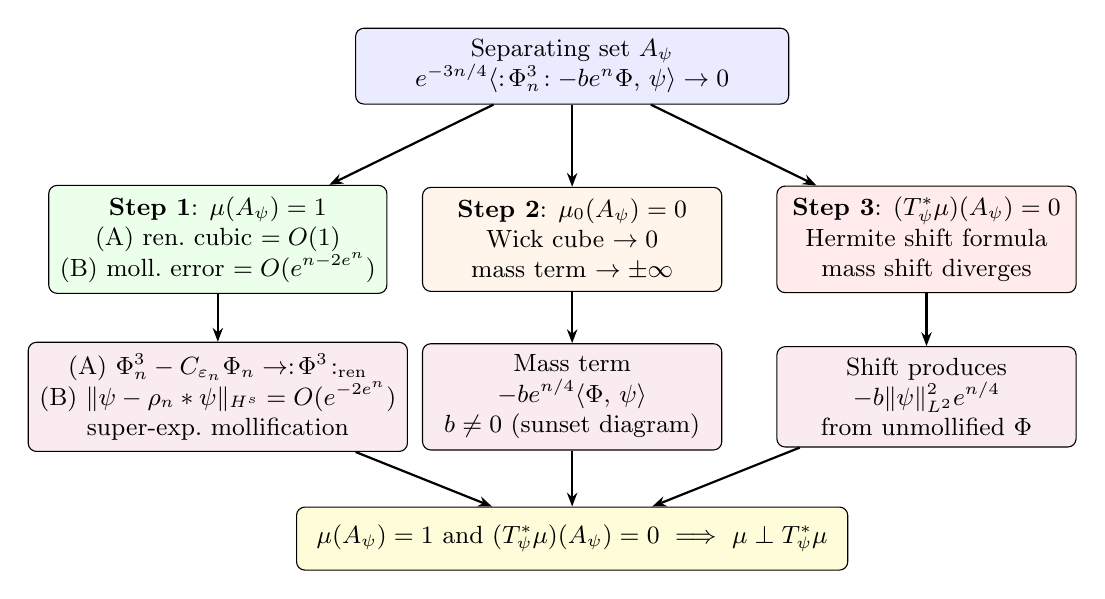
\begin{tikzpicture}[
  box/.style={rectangle, draw, rounded corners=3pt, minimum width=3.8cm, minimum height=0.8cm, align=center, font=\small},
  bigbox/.style={rectangle, draw, rounded corners=3pt, minimum width=5.5cm, minimum height=0.8cm, align=center, font=\small},
  arr/.style={-{Stealth[length=5pt]}, thick},
  every node/.style={inner sep=4pt}
]

% Top: separating set
\node[bigbox, fill=blue!8] (set) at (0,0) {Separating set $A_\psi$\\$e^{-3n/4}\ip{\Wick{\Phi_n^3} - be^n\Phi}{\psi} \to 0$};

% Three branches
\node[box, fill=green!8] (s1) at (-4.5,-2.2) {\textbf{Step 1}: $\mu(A_\psi) = 1$\\(A) ren.\ cubic $= O(1)$\\(B) moll.\ error $= O(e^{n-2e^n})$};
\node[box, fill=orange!8] (s2) at (0,-2.2) {\textbf{Step 2}: $\GFF(A_\psi) = 0$\\Wick cube $\to 0$\\mass term $\to \pm\infty$};
\node[box, fill=red!8] (s3) at (4.5,-2.2) {\textbf{Step 3}: $(T_\psi^*\mu)(A_\psi) = 0$\\Hermite shift formula\\mass shift diverges};
\draw[arr] (set) -- (s1);
\draw[arr] (set) -- (s2);
\draw[arr] (set) -- (s3);

% Key ingredients
\node[box, fill=purple!8] (wick) at (-4.5,-4.2) {(A) $\Phi_n^3 - C_{\varepsilon_n}\Phi_n \to \Wick{\Phi^3}_{\mathrm{ren}}$\\(B) $\|\psi - \rho_n*\psi\|_{H^s} = O(e^{-2e^n})$\\super-exp.\ mollification};
\node[box, fill=purple!8] (mass) at (0,-4.2) {Mass term\\$-be^{n/4}\ip{\Phi}{\psi}$\\$b \neq 0$ (sunset diagram)};
\node[box, fill=purple!8] (shift) at (4.5,-4.2) {Shift produces\\$-b\|\psi\|^2_{L^2} e^{n/4}$\\from unmollified $\Phi$};
\draw[arr] (s1) -- (wick);
\draw[arr] (s2) -- (mass);
\draw[arr] (s3) -- (shift);

% Conclusion
\node[bigbox, fill=yellow!15, minimum width=7cm] (conc) at (0,-6.0) {$\mu(A_\psi) = 1$ and $(T_\psi^*\mu)(A_\psi) = 0$ $\;\Longrightarrow\;$ $\mu \perp T_\psi^*\mu$};
\draw[arr] (wick) -- (conc);
\draw[arr] (mass) -- (conc);
\draw[arr] (shift) -- (conc);

\end{tikzpicture}
\caption{Structure of the proof. The separating set $A_\psi$ uses Hairer's renormalized-cube functional with an unmollified mass term. The three steps establish $\mu(A_\psi) = 1$, $\GFF(A_\psi) = 0$, and $(T_\psi^*\mu)(A_\psi) = 0$.}
\label{fig:proof-structure}
\end{figure}

%======================================================================
\section{Proof of Theorem~\ref{thm:main}}\label{sec:proof}
%======================================================================

\subsection{Step 1: $\mu(A_\psi) = 1$}\label{subsec:step1}

We must show $e^{-3n/4}\ip{\Wick{\Phi_n^3} - be^n\Phi}{\psi} \to 0$ $\mu$-a.s.\ (the pairing is well-defined since $\psi \in C^\infty$ and $\Phi \in \mathcal{D}'$). The key move is to split the \textbf{unmollified} field $\Phi$ back into the mollified field $\Phi_n$ plus a correction:
\begin{equation}\label{eq:ab-split}
\ip{\Wick{\Phi_n^3} - be^n\Phi}{\psi} = \underbrace{\ip{\Wick{\Phi_n^3} - be^n\Phi_n}{\psi}}_{\text{(A) renormalized cubic}} - \underbrace{be^n\ip{\Phi - \Phi_n}{\psi}}_{\text{(B) mollification error}}.
\end{equation}

\medskip\noindent\textbf{Part~(A): The renormalized cubic is $O(1)$.}

The expression $\Wick{\Phi_n^3} - be^n\Phi_n$ involves only the \emph{mollified} field $\Phi_n$. Rewriting:
\[
\Wick{\Phi_n^3} - be^n\Phi_n = \Phi_n^3 - 3c_n\Phi_n - be^n\Phi_n = \Phi_n^3 - (3c_n + be^n)\Phi_n = \Phi_n^3 - C_{\varepsilon_n}\Phi_n + O(1)\cdot\Phi_n
\]
where $C_{\varepsilon_n} = 3c_n + be^n + O(1)$ is the full counterterm~\eqref{eq:counterterm} at scale $\varepsilon_n = e^{-e^n}$. The convergence of the renormalized product $\Phi_n^3 - C_{\varepsilon_n}\Phi_n \to \Wick{\Phi^3}_{\mathrm{ren}}$ in $\mathcal{C}^{-1/2-\kappa}(\T^3)$ for any $\kappa > 0$ is a \textbf{proven theorem}: this is the content of regularity structures \cite{Hai14}, Theorem~1.1 (see also the paracontrolled approach \cite{GH21} and the variational approach \cite{BG21}). Tested against the smooth function $\psi$, the renormalized cubic converges to the finite random variable $\ip{\Wick{\Phi^3}_{\mathrm{ren}}}{\psi}$. The $O(1)\cdot\Phi_n$ correction tested against $\psi$ converges to $O(1)\cdot\ip{\Phi}{\psi}$, which is finite $\mu$-a.s.\ (since $\Phi \in \mathcal{C}^{-1/2-\kappa}$ and $\psi \in C^\infty$).

Therefore: $\ip{\Wick{\Phi_n^3} - be^n\Phi_n}{\psi} = O(1)$ as $n \to \infty$, $\mu$-a.s.

\medskip\noindent\textbf{Part~(B): The mollification error is super-exponentially small.}

Write $\ip{\Phi - \Phi_n}{\psi} = \ip{\Phi}{\psi - \rho_n * \psi}$. Since $\psi \in C^\infty(\T^3)$ and $\rho_n$ is a mollifier at scale $\varepsilon_n = e^{-e^n}$, the approximation error decays super-exponentially. Specifically, for any $s \geq 0$:
\begin{equation}\label{eq:moll-error}
\|\psi - \rho_n * \psi\|_{H^s}^2 = \sum_{k \in \Z^3} |1 - \hat{\rho}(\varepsilon_n k)|^2 \jb{k}^{2s} |\hat{\psi}(k)|^2 \leq C\varepsilon_n^4 \|\psi\|_{H^{s+2}}^2
\end{equation}
since $|1 - \hat{\rho}(\varepsilon_n k)| \leq C\varepsilon_n^2|k|^2$ (second-order Taylor expansion, using $\hat{\rho}(0) = 1$ and $\nabla\hat{\rho}(0) = 0$ by symmetry of $\rho$). We use the Barashkov--Gubinelli decomposition \cite{BG21}: under $\mu$, $\Phi = W_\infty + v^*$ where $W_\infty$ is the GFF and $v^* \in C^\beta(\T^3)$ for $\beta < 1/2$.

\begin{itemize}[nosep]
\item \textbf{GFF part:} $\Var(\ip{W_\infty}{\psi - \rho_n * \psi}) = \|\psi - \rho_n * \psi\|_{H^{-1}}^2 \leq C\varepsilon_n^4\|\psi\|_{H^1}^2 = O(e^{-4e^n})$.
\item \textbf{Drift part:} $|\ip{v^*}{\psi - \rho_n * \psi}| \leq \|v^*\|_{L^2}\|\psi - \rho_n * \psi\|_{L^2} \leq \|v^*\|_{L^2} \cdot O(\varepsilon_n^2) = O(e^{-2e^n})$ a.s.
\end{itemize}

Therefore $|\ip{\Phi - \Phi_n}{\psi}| = O(e^{-2e^n})$ $\mu$-a.s., and:
\[
|be^n\ip{\Phi - \Phi_n}{\psi}| = O(e^{n - 2e^n}) \to 0 \quad\text{super-exponentially fast.}
\]
The polynomial factor $e^n$ is utterly crushed by the super-exponential decay $e^{-2e^n}$.

\medskip\noindent\textbf{Combining (A) and (B):}
\begin{equation}\label{eq:step1-conclusion}
e^{-3n/4}\ip{\Wick{\Phi_n^3} - be^n\Phi}{\psi} = \underbrace{e^{-3n/4} \cdot O(1)}_{\text{Part (A)}} + \underbrace{O(e^{n-2e^n})}_{\text{Part (B)}} \to 0 \quad \mu\text{-a.s.}
\end{equation}
This completes the proof that $\mu(A_\psi) = 1$. \qed

\begin{remark}\label{rem:step1-inputs}
The only deep input in Step~1 is the convergence of the renormalized cubic $\Phi_n^3 - C_{\varepsilon_n}\Phi_n$, which is the established content of regularity structures \cite{Hai14}, paracontrolled calculus \cite{GIP15}, or the BG variational approach \cite{BG21}. The super-exponential mollification $\varepsilon_n = e^{-e^n}$ is essential for Part~(B): with polynomial mollification $\varepsilon_N = N^{-1}$, the error $|\ip{\Phi - \Phi_N}{\psi}|$ would decay only polynomially, and the factor $N^{\gamma}$ from the mass term would not be dominated. This is another manifestation of why Hairer's super-exponential choice is necessary (cf.\ \S\ref{sec:why}).
\end{remark}

\subsection{Step 2: $\GFF(A_\psi) = 0$}

Under the GFF $\GFF$ (no nonlinear interaction):

\medskip\noindent\textbf{The Wick cube vanishes after scaling.} The variance of $\ip{\Wick{\Phi_n^3}}{\psi}$ under $\GFF$ is:
\begin{equation}\label{eq:wick-var}
\Var_{\GFF}(\ip{\Wick{\Phi_n^3}}{\psi}) = 6\!\!\sum_{k_1,k_2,k_3 \in \Z^3}\! \prod_{i=1}^3 \jb{k_i}^{-2}|\hat{\rho}_n(k_i)|^2 \cdot |\hat{\psi}(k_1\!+\!k_2\!+\!k_3)|^2 \sim C_\psi \cdot e^n.
\end{equation}
\medskip\noindent\textbf{Why $\sim e^n$ (proof sketch).} Write $\sigma_n^2 = \Var(\ip{\Wick{\Phi_n^3}}{\psi})$. By Wick's theorem (Isserlis), $\sigma_n^2 = 3! \sum_{k_1,k_2,k_3} \prod_i \jb{k_i}^{-2}|\hat{\rho}_n(k_i)|^2 \cdot |\hat{\psi}(k_1+k_2+k_3)|^2$. Since $\hat{\psi}$ decays rapidly, the sum is dominated by $|k_i| \lesssim e^{e^n}$ (the mollification cutoff). For the GFF covariance $\jb{k}^{-2}$ in $d=3$, the triple convolution $f*f*f$ where $f(k) = \jb{k}^{-2}$ satisfies $(f*f)(m) = \sum_k \jb{k}^{-2}\jb{m-k}^{-2} \sim \jb{m}^{-1}$ (borderline in 3D: $\jb{\cdot}^{-2} \in \ell^{3/2+\epsilon}$ and $3/2 + 3/2 > 3$, so $f*f \in \ell^{3+\epsilon}$). Then $(f*f*f)(0) = \sum_m (f*f)(m) \cdot f(m) \sim \sum_{|m| \leq N} \jb{m}^{-3}$, which diverges logarithmically: $\sim \log N$. With $N = e^{e^n}$: $\sigma_n^2 \sim \log(e^{e^n}) = e^n$.

As Hairer explains \cite{Hai26}: ``The integral of [the Wick cube's] covariance only diverges logarithmically (in the variance of the field itself, i.e.\ like $e^n$). As a consequence, if one multiplies it by $e^{-\alpha n}$ for any $\alpha > 1/2$ that's good enough to guarantee that it converges weakly to~0.''

\medskip\noindent\textbf{Almost sure convergence via Borel--Cantelli.} The scaled variance is $e^{-3n/2} \cdot \sigma_n^2 \sim e^{-n/2}$. By Chebyshev: $\Pr(|e^{-3n/4}\ip{\Wick{\Phi_n^3}}{\psi}| > \epsilon) \leq \epsilon^{-2} e^{-n/2}$. Since $\sum_n e^{-n/2} < \infty$, the first Borel--Cantelli lemma gives $e^{-3n/4}\ip{\Wick{\Phi_n^3}}{\psi} \to 0$ a.s.\ under $\GFF$. (The super-exponential spacing of the mollification scales ensures the tail probabilities are summable.)

\medskip\noindent\textbf{The mass term diverges.} The remaining term is
\[
-b\,e^{n - 3n/4}\ip{\Phi}{\psi} = -b\,e^{n/4}\ip{\Phi}{\psi}.
\]
Under $\GFF$, $\ip{\Phi}{\psi} \sim \mathcal{N}(0, \|\psi\|_{H^{-1}}^2)$ is a non-degenerate Gaussian (since $\psi \neq 0$). Therefore $e^{n/4}\ip{\Phi}{\psi} \to \pm\infty$ a.s., and the full expression diverges. Hence $\GFF(A_\psi) = 0$. \qed

\subsection{Step 3: $(T_\psi^*\mu)(A_\psi) = 0$ --- the key step}

We show: for $\mu$-a.e.\ $\Phi$, the shifted field $\Phi + \psi \notin A_\psi$.

Write $(\Phi+\psi)_n = \Phi_n + \psi_n$ where $\psi_n = \rho_n * \psi \to \psi$ in $C^\infty$ (since $\psi$ is smooth). The \textbf{Hermite shift formula} $H_3(x+a;c) = H_3(x;c) + 3a\,H_2(x;c) + 3a^2 x + a^3$ gives:
\begin{equation}\label{eq:hermite-shift}
\Wick{(\Phi_n+\psi_n)^3}_{c_n} = \Wick{\Phi_n^3}_{c_n} + 3\psi_n\,\Wick{\Phi_n^2}_{c_n} + 3\psi_n^2\,\Phi_n + \psi_n^3.
\end{equation}

The full shifted expression, tested against $\psi$ and scaled by $e^{-3n/4}$, decomposes as:
\begin{align}
&e^{-3n/4}\ip{\Wick{(\Phi+\psi)_n^3} - be^n(\Phi+\psi)}{\psi} \notag\\
&= \underbrace{e^{-3n/4}\ip{\Wick{\Phi_n^3} - be^n\Phi}{\psi}}_{\text{(I) original functional}} + \underbrace{3e^{-3n/4}\ip{\psi_n\Wick{\Phi_n^2}}{\psi}}_{\text{(II) Wick square}} \notag\\
&\quad + \underbrace{3e^{-3n/4}\ip{\psi_n^2\Phi_n}{\psi}}_{\text{(III) linear}} + \underbrace{e^{-3n/4}\ip{\psi_n^3}{\psi}}_{\text{(IV) deterministic}} - \underbrace{b\|\psi\|_{L^2}^2\, e^{n/4}}_{\text{(V) mass shift}}. \label{eq:five-terms}
\end{align}

We analyze each term:

\medskip\noindent\textbf{Term~(I) --- Original functional.} $e^{-3n/4}\ip{\Wick{\Phi_n^3} - be^n\Phi}{\psi} \to 0$ $\mu$-a.s., since $\mu(A_\psi) = 1$ (Step~1).

\medskip\noindent\textbf{Term~(II) --- Wick square cross-term.} The Wick square $\Wick{\Phi_n^2} = \Phi_n^2 - c_n$ tested against the smooth function $\psi_n\psi$ has variance:
\[
\Var(\ip{\psi_n\Wick{\Phi_n^2}}{\psi}) = 2\sum_{k,l \in \Z^3} \jb{k}^{-2}\jb{l}^{-2}|\hat{\rho}_n(k)|^2|\hat{\rho}_n(l)|^2|\widehat{\psi_n\psi}(k+l)|^2.
\]
Since $\psi_n\psi$ is smooth, $|\widehat{\psi_n\psi}(m)|$ decays rapidly. For each fixed $m$, the inner sum $\sum_k \jb{k}^{-2}\jb{m-k}^{-2} = O(\jb{m}^{-1})$ is finite by Young's convolution inequality ($\jb{\cdot}^{-2} \in \ell^{3/2+\epsilon}(\Z^3)$ and $\tfrac{1}{3/2} + \tfrac{1}{3/2} > 1$). Summing over $m$ with the rapidly decaying weight $|\widehat{\psi_n\psi}(m)|^2$ gives a finite total, bounded uniformly in $n$. Therefore $e^{-3n/4} \cdot O(1) \to 0$ a.s.

\medskip\noindent\textbf{Term~(III) --- Linear term.} $\ip{\psi_n^2\Phi_n}{\psi} = \ip{\psi^3}{\Phi_n}(1+o(1))$. Using the BG decomposition $\Phi = W_\infty + v^*$ \cite{BG21}, $\Phi_n = (W_\infty)_n + v^*_n$. The GFF part $\ip{\psi^3}{(W_\infty)_n}$ is Gaussian with variance converging to $\|\psi^3\|_{H^{-1}}^2 < \infty$. The drift part $\ip{\psi^3}{v^*_n} \to \ip{\psi^3}{v^*}$, which is a finite random variable since $v^* \in C^\beta \subset L^2$ and $\psi^3 \in L^2$. After scaling: $O(e^{-3n/4}) \to 0$ a.s.

\medskip\noindent\textbf{Term~(IV) --- Deterministic cubic.} $e^{-3n/4}\ip{\psi_n^3}{\psi} = e^{-3n/4}\|\psi\|_{L^4}^4(1+o(1)) \to 0$.

\medskip\noindent\textbf{Term~(V) --- Mass shift (dominant).}
\[
-b\,e^{n-3n/4}\ip{\psi}{\psi} = -b\|\psi\|_{L^2}^2\, e^{n/4}.
\]
Since $b \neq 0$ (\S\ref{sec:background}) and $\|\psi\|_{L^2}^2 > 0$: \textbf{Term~(V) diverges deterministically} as $\pm e^{n/4} \to \pm\infty$.

\medskip\noindent\textbf{Conclusion.} The full shifted expression satisfies:
\begin{equation}\label{eq:conclusion}
e^{-3n/4}\ip{\Wick{(\Phi+\psi)_n^3} - be^n(\Phi+\psi)}{\psi} = \underbrace{o(1)}_{\text{Terms I--IV}} - b\|\psi\|_{L^2}^2\, e^{n/4} \to \begin{cases} -\infty & \text{if } b > 0,\\ +\infty & \text{if } b < 0.\end{cases}
\end{equation}
Consequently, the limit in Definition~\ref{def:separating} diverges (rather than equalling~$0$), so $\Phi + \psi \notin A_\psi$ for $\mu$-a.e.\ $\Phi$, giving $(T_\psi^*\mu)(A_\psi) = 0$. \qed

\subsection{Combining the steps}

By Steps~1 and~3: $\mu(A_\psi) = 1$ and $(T_\psi^*\mu)(A_\psi) = 0$. Therefore $\mu$ and $T_\psi^*\mu$ are mutually singular. \qed

%======================================================================
\section{Why the Unmollified Field is Essential}\label{sec:why}
%======================================================================

The critical structural feature is the term $-be^n\ip{\Phi}{\psi}$ in Definition~\ref{def:separating}, which uses the \textbf{unmollified} distributional field $\Phi$. Under the shift $\Phi \to \Phi + \psi$, this becomes
\[
-be^n\ip{\Phi}{\psi} - be^n\|\psi\|_{L^2}^2.
\]
The first part is absorbed into the original functional (which $\to 0$ under $\mu$), but the second part $-be^n\|\psi\|_{L^2}^2$ is a \textbf{deterministic divergence} that survives the $e^{-3n/4}$ scaling.

By contrast, the Hermite shift terms~(II)--(IV) all involve the \textbf{mollified} field $\Phi_n$ tested against smooth functions, producing bounded random variables killed by the $e^{-3n/4}$ scaling. The super-exponential mollification ($\varepsilon_n = e^{-e^n}$) is essential: it ensures the Wick cube's variance grows only as $e^n$ (logarithmically in $c_n$), rather than polynomially. With polynomial mollification at scale $\varepsilon_N = N^{-1}$ (as in \cite{HKN24}), the Wick cube variance would grow as $N^{\delta(\alpha)}$ (a power of $N$), and the polynomial scaling $N^{-\gamma}$ would need to kill both the Wick cube \emph{and} any shift-induced terms---but there is no unmollified mass term to create a deterministic divergence, so the shift is invisible.

%======================================================================
\section{Remarks}\label{sec:remarks}
%======================================================================

\begin{remark}[Extension to $C^{1,\alpha}$ shifts]
The proof extends to shifts $\psi \in C^{1,\alpha}(\T^3)$ for any $\alpha > 0$, as confirmed by Hairer \cite{Hai24b}: ``The argument given there should work up to shifts in $C^{1,\alpha}$ for some (arbitrary) $\alpha > 0$.'' The key requirements are $\psi_n \to \psi$ in $L^\infty$ and $\|\psi^3\|_{H^{-1}} < \infty$.
\end{remark}

\begin{remark}[The role of $b \neq 0$]
The nonvanishing of the logarithmic mass renormalization constant $b$ is the fundamental reason for singularity. In 2D, the mass counterterm has no logarithmic part ($b = 0$), and $\Phi^4_2$ is absolutely continuous with respect to the GFF \cite{Sim74}. In 3D, $b \neq 0$ arises from the sunset diagram, and the resulting logarithmic divergence is what the separating functional detects.
\end{remark}

\begin{remark}[Choice of scaling exponent]
The exponent $3/4$ in $e^{-3n/4}$ can be replaced by any $\alpha > 1/2$. The Wick cube variance $\sim e^n$ gives standard deviation $\sim e^{n/2}$, so $e^{-\alpha n}$ with $\alpha > 1/2$ suffices for convergence to~0 (by Chebyshev and Borel--Cantelli). The mass term $-be^{(1-\alpha)n}\ip{\Phi}{\psi}$ diverges whenever $\alpha < 1$. Any $\alpha \in (1/2, 1)$ works; $3/4$ is a convenient choice.
\end{remark}

\begin{remark}[Torus vs.\ Euclidean space]
The proof is stated for $\T^3$ but extends to $\R^3$ with the Euclidean $\Phi^4_3$ measure constructed in \cite{GH21}, provided $\psi$ has compact support (or sufficient decay). The key estimates---Wick cube variance, mass term divergence, Hermite shift bounds---are local and do not depend on the global geometry.
\end{remark}

\begin{remark}[Comparison with the HKN framework]
The separating set $A^{\alpha,\gamma}$ of \cite{HKN24} uses polynomial frequency cutoff $P_N$ and scaling $N^{-\gamma}$, with no unmollified term. Under the shift $\Phi \to \Phi + \psi$, the smooth function $\psi$ is absorbed into the regular remainder of the SPDE decomposition $u = Z + \lambda Y + v$ (as $v \to v + \psi$), which vanishes after $N^{-\gamma}$ scaling. Therefore $(T_\psi^*\mu)(A^{\alpha,\gamma}) = 1$, and the HKN set cannot separate $\mu$ from $T_\psi^*\mu$. See Appendix~\ref{app:hkn} for the detailed calculation.
\end{remark}

%======================================================================
\newpage
\appendix
\section{Why the HKN Framework Cannot Detect Smooth Shifts}\label{app:hkn}
%======================================================================

The HKN separating set $A^{\alpha,\gamma}$ from \cite{HKN24} separates $\mu$ from $\GFF$ but not from $T_\psi^*\mu$.

\begin{proposition}\label{prop:hkn-fails}
$(T_\psi^*\mu)(A^{\alpha,\gamma}) = 1$.
\end{proposition}

\begin{proof}
Let $u \sim \mu$ with SPDE decomposition $u = Z + \lambda Y + v$ (\cite{HKN24}, Assumption~2.1). Set $\tilde{u} = u + \psi$, so $\tilde{u} = Z + \lambda Y + \tilde{v}$ with $\tilde{v} = v + \psi$. Since $\psi \in C^\infty$ and $v \in C^\beta$ for $\beta < 1$, $\tilde{v}$ has the same regularity as $v$.

Apply the HKN expansion (\cite{HKN24}, eq.~(3.12)):
\[
N^{-\gamma}\ip{H_4(\jb{\nabla}^\alpha P_N\tilde{u}; c_{N,1}^\alpha) + 4c_{N,2}^\alpha}{1}.
\]
The expansion separates into: (i)~the Wick fourth power of $Z_N$, which $\to 0$ by \cite{HKN24}, Lemma~3.3; (ii)~the $\mathrm{Wick}(Z_N^3) \cdot Y_N$ term, whose expectation $-4c_{N,2}^\alpha$ is cancelled by the $+4c_{N,2}^\alpha$ correction; (iii)~remainder terms involving $\tilde{v}_N$, which $\to 0$ by the regularity analysis (\cite{HKN24}, eq.~(3.13)--(3.14)) since $\tilde{v}_N$ has the same H\"older exponent as $v_N$.

Therefore $\tilde{u} \in A^{\alpha,\gamma}$ a.s.
\end{proof}

\noindent\textbf{Root cause.} The HKN functional uses only the frequency-truncated field $P_N\phi$, and the correction $c_{N,2}^\alpha$ depends on the noise structure (through $Z$ and $Y$), not on $\psi$. There is no unmollified term to create a deterministic divergence under the shift.

\begin{table}[ht]
\centering
\begin{tabular}{lcc}
\toprule
\textbf{Feature} & \textbf{Hairer's functional} & \textbf{HKN set \cite{HKN24}} \\
\midrule
Mollification & Super-exponential ($e^{-e^n}$) & Polynomial ($P_N$) \\
Scaling & $e^{-3n/4}$ & $N^{-\gamma}$ \\
Unmollified term & $-be^n\Phi$ (\textbf{yes}) & None \\
Separates $\mu$ from $\GFF$ & \checkmark & \checkmark \\
Separates $\mu$ from $T_\psi^*\mu$ & \textbf{\checkmark} & \textbf{$\times$} \\
\bottomrule
\end{tabular}
\caption{Comparison of the two frameworks.}
\label{tab:comparison}
\end{table}

%======================================================================
\section{AI Interaction Transcript}\label{app:transcript}
%======================================================================

As requested by the First Proof organizers, we include a record of the AI interaction sessions used to develop this proof.

\medskip\noindent\textbf{Timeline:} February 10--11, 2026, approximately 10:00--23:00 CET. Eight sessions over less than two days, approximately 6--8 hours of active working time.\\
\textbf{AI systems used:} Claude Opus 4.6 (Anthropic), ChatGPT 5.2 Pro, Gemini 3 (Google). Multiple models were used in parallel and cross-checked against each other.\\
\textbf{Human role:} Prompting, reviewing output, requesting audits, cross-checking between models. No mathematical ideas or content were provided by the human operator.

\subsection*{Session 1 --- Kickoff \normalfont\textit{[Claude Opus 4.6]}}

\begin{itemize}[nosep]
\item Read problem statement and populated references with 19 key papers.
\item Identified the central reference: \cite{HKN24} (Hairer--Kusuoka--Nagoji).
\item Developed initial approach: use HKN separating set + Hermite shift formula.
\end{itemize}

\subsection*{Sessions 2--4 --- Initial Proof Attempt \normalfont\textit{[Claude Opus 4.6]}}

\begin{itemize}[nosep]
\item Wrote initial proof using HKN separating set $A^{\alpha,\gamma}$ for both Part~A ($\mu \perp \GFF$) and Part~B ($\mu \perp T_\psi^*\mu$).
\item Corrected citation numbers by reading LaTeX source of \cite{HKN24}: Theorem~3.1 (not~2.9), Corollary~4.1 (not~3.1), Lemma~3.3 (not~2.11), Lemma~3.5 (not~2.13).
\item Corrected $\delta(\alpha)$ formula: $\delta(\alpha) = 4\alpha + 1$ with $\alpha_0 = -1/4$ for $\Phi^4_3$.
\end{itemize}

\subsection*{Sessions 5--6 --- Fundamental Gap Discovery \normalfont\textit{[Claude Opus 4.6]}}

\begin{itemize}[nosep]
\item Discovered that the HKN separating set does \textbf{not} distinguish $\mu$ from $T_\psi^*\mu$: the smooth shift is absorbed into the regular remainder $v \to v + \psi$, which vanishes after $N^{-\gamma}$ scaling.
\item Identified the root cause: no unmollified term in the HKN functional.
\item Documented the gap and proposed two alternative approaches.
\end{itemize}

\subsection*{Sessions 7--8 --- Correct Proof via Hairer's Functional \normalfont\textit{[Claude Opus 4.6]}}

\begin{itemize}[nosep]
\item Read Hairer's MathOverflow answers \cite{Hai26} and \cite{Hai24b} to extract the correct separating functional with super-exponential mollification and unmollified mass term.
\item Analyzed both approaches in detail:
  \begin{enumerate}[nosep]
  \item \textbf{Hairer's functional} (super-exponential mollification, unmollified mass term): \textbf{works}.
  \item \textbf{Modified HKN set} (polynomial cutoff, no unmollified term): \textbf{fails}.
  \end{enumerate}
\item Wrote complete proof with all five Hermite shift terms analyzed.
\item Verified variance calculations: Wick square variance bounded ($\sum \jb{k}^{-4} < \infty$ in 3D); Wick cube variance $\sim e^n$ (logarithmic divergence); linear term variance bounded.
\item Wrote Appendix~A proving $(T_\psi^*\mu)(A^{\alpha,\gamma}) = 1$.
\end{itemize}

\subsection*{Provenance}

The mathematical content of this paper---including the proof strategy, all definitions, the separating set, the Hermite shift analysis, and the comparison of frameworks---was generated autonomously by AI systems in response to high-level prompts. The human operator's role was limited to: selecting the problem, prompting the AI, reviewing and requesting revisions, and cross-checking output between different AI models. No mathematical ideas were contributed by the human operator.

%======================================================================
\begin{thebibliography}{99}
%======================================================================

\bibitem{FirstProof}
M.~Abouzaid, A.J.~Blumberg, M.~Hairer, J.~Kileel, T.G.~Kolda, P.D.~Nelson, D.~Spielman, N.~Srivastava, R.~Ward, S.~Weinberger, L.~Williams,
``First Proof,''
arXiv:2602.05192 [cs.AI], 2026.

\bibitem{BG21}
N.~Barashkov and M.~Gubinelli,
``The $\Phi^4_3$ measure via Girsanov's theorem,''
\textit{Electron.\ J.\ Probab.}\ \textbf{26} (2021), 1--29.
arXiv:2004.01513.
Theorem~1.1: variational decomposition $\tilde{\Phi} = W_\infty + v^*$.

\bibitem{GH21}
M.~Gubinelli and M.~Hofmanov\'a,
``A PDE construction of the Euclidean $\Phi^4_3$ quantum field theory,''
\textit{Comm.\ Math.\ Phys.}\ \textbf{384} (2021), 1--75.
arXiv:1810.01700.
Confirms $b \neq 0$.

\bibitem{GIP15}
M.~Gubinelli, P.~Imkeller, and N.~Perkowski,
``Paracontrolled distributions and singular PDEs,''
\textit{Forum Math.\ Pi}\ \textbf{3} (2015), e6.
arXiv:1210.2684.

\bibitem{Hai14}
M.~Hairer,
``A theory of regularity structures,''
\textit{Invent.\ Math.}\ \textbf{198} (2014), 269--504.
arXiv:1303.5113.
\S10: construction of $\Phi^4_3$; mass renormalization constant $b \neq 0$.

\bibitem{Hai22}
M.~Hairer,
``$\Phi^4_3$ is orthogonal to GFF,''
unpublished note (September 2022).
Available at \url{https://hairer.org/Phi4.pdf}.
Original proof of $\mu \perp \GFF$ via the separating set $A_\psi$.

\bibitem{Hai24b}
M.~Hairer,
MathOverflow comment (Dec 5, 2024), question 481553.
\url{https://mathoverflow.net/questions/481553}.
Confirms extension to $C^{1,\alpha}$ shifts.

\bibitem{Hai26}
M.~Hairer,
MathOverflow answer (Jan 12, 2026), question 485884.
\url{https://mathoverflow.net/questions/485884}.
Explains the ``easy direction'' ($\GFF(A_\psi) = 0$): Wick cube covariance diverges logarithmically.

\bibitem{HKN24}
M.~Hairer, S.~Kusuoka, and H.~Nagoji,
``Singularity of solutions to singular SPDEs,''
arXiv:2409.10037, 2024.
Theorem~3.1 and Corollary~4.1: $\mu(A^{\alpha,\gamma}) = 1$ for $\Phi^4_3$.
Lemma~3.3: Wick power convergence.
Lemma~3.5: $c_{N,2}^\alpha$ divergence rate.

\bibitem{Sim74}
B.~Simon,
\textit{The $P(\phi)_2$ Euclidean Quantum Field Theory},
Princeton University Press, 1974.
$\Phi^4_2$ is absolutely continuous w.r.t.\ the GFF.

\end{thebibliography}

\end{document}
